\documentclass[12pt, a4paper]{article} % book, report, article, letter, slides
                                       % letterpaper/a4paper, 10pt/11pt/12pt, twocolumn/twoside/landscape/draft

%%%%%%%%%%%%%%%% PACKAGES %%%%%%%%%%%%%%%%%%%%%

\usepackage[utf8]{inputenc} % encoding

\usepackage[english]{babel} % use special characters and also translates some elements within the document.

\usepackage{amsmath}        % Math
\usepackage{amsthm}         % Math, \newtheorem, \proof, etc
\usepackage{amssymb}        % Math, extended collection
\newtheorem{theorem}{Theorem}[section]     % \begin{theorem}\label{t:label}  \end{theorem}<Paste>
\newtheorem{corollary}{Corollary}[theorem]
\newtheorem{lemma}[theorem]{Lemma}
\DeclareMathOperator*{\argmax}{arg\,max}
\DeclareMathOperator*{\argmin}{arg\,min}

\usepackage{hyperref}       % Hyperlinks \url{url} or \href{url}{name}

\usepackage{parskip}        % \par starts on left (not idented)

\usepackage{abstract}       % Abstract

\usepackage{tocbibind}      % Adds the bibliography to the table of contents (automatically)

\usepackage{graphicx}       % Images
\graphicspath{ {./images/} }

% \usepackage[document]{ragged2e}  % Left-aligned (whole document)
% \begin{...} ... \end{...}   flushleft, flushright, center

%%%%%%%%%%%%%%%% CODE %%%%%%%%%%%%%%%%%%%%%

\usepackage{minted}         % Code listing
% \mint{html}|<h2>Something <b>here</b></h2>|
% \inputminted{octave}{BitXorMatrix.m}

%\begin{listing}[H]
  %\begin{minted}[xleftmargin=20pt,linenos,bgcolor=codegray]{haskell}
  %\end{minted}
  %\caption{Example of a listing.}
  %\label{lst:example} % You can reference it by \ref{lst:example}
%\end{listing}

\newcommand{\code}[1]{\texttt{#1}} % Define \code{foo.hs} environment

%%%%%%%%%%%%%%%% COLOURS %%%%%%%%%%%%%%%%%%%%%

\usepackage{xcolor}         % Colours \definecolor, \color{codegray}
\definecolor{codegray}{rgb}{0.9, 0.9, 0.9}
% \color{codegray} ... ...
% \textcolor{red}{easily}

%%%%%%%%%%%%%%%% CONFIG %%%%%%%%%%%%%%%%%%%%%

\renewcommand{\absnamepos}{flushleft}
\setlength{\absleftindent}{0pt}
\setlength{\absrightindent}{0pt}

%%%%%%%%%%%%%%%% GLOSSARIES %%%%%%%%%%%%%%%%%%%%%

%\usepackage{glossaries}

%\makeglossaries % before entries

%\newglossaryentry{latex}{
    %name=latex,
    %description={Is a mark up language specially suited
    %for scientific documents}
%}

% Referene to a glossary \gls{latex}
% Print glossaries \printglossaries

\usepackage[ruled]{algorithm2e} % pseudo-code  linesnumbered

%%%%%%%%%%%%%%%% HEADER %%%%%%%%%%%%%%%%%%%%%

\usepackage{fancyhdr}
\pagestyle{fancy}
\fancyhf{}
\rhead{Arnau Abella}
\lhead{MIRI - Algorithms for Data Mining}
\rfoot{Page \thepage}

%%%%%%%%%%%%%%%% TITLE %%%%%%%%%%%%%%%%%%%%%

\title{%
  Optimized K-Means Clustering Algorithm in Haskell\\
}
\author{%
  Arnau Abella \\
  \large{Universitat Polit\`ecnica de Catalunya}
}
\date{\today}

%%%%%%%%%%%%%%%% DOCUMENT %%%%%%%%%%%%%%%%%%%%%

\begin{document}

\maketitle

\section{Introduction}\label{s:intro}

The \textit{k-means} clustering algorithm aims to partition $n$ observations into $k$ clusters in which each observation belongs to the cluster with the \textit{nearest mean} (cluster centers or cluster centroid), serving as a prototype of the cluster. This results in a partitioning of the data space into \textit{Voronoi cells}. It is popular for cluster analysis in data mining.

This paper describes an \textit{optimized} implementation in Haskell, the purely funcitonal programming language, of the \textit{standard k-means clustering} algorithm, see algorithm \ref{algo:kmeans}. This project also provides a \textit{library} with a very simple API to use. Furthemore, it include a couple of utils to plot the result of the clustering, see in figure \ref{fig:kmeans}.

\subsection{The algorithm}\label{s:algo}

Given a set of observations $(x_1, \dots, x_n)$, where each observation is a $d$-dimensional real vector, $k$-means clustering aims to partition the $n$ observations into $k \leq n$ sets, $S = (S_1, \dots, S_k)$, so as to minimize the \textit{within-cluster sum of squares (WCSS)}. Formally, the objective is to find:

\begin{equation}\label{eq:objective}
  \argmin_{S} \sum_{i=1}^k \sum_{x \in S_i} {\|x - \mu_i\|}^2
\end{equation}

The algorithm implementation is \textit{straightforward} and it can be easily implemented in any turing-complete programming language \cite{mohammed}.

\begin{algorithm}[h]
  1. Choose k data objects representing the cluster centroids \\
  2. Assign each data objet of the entire data set to the cluster having the closest centroid \\
  3. Compute new centroid for each cluster, by averaging the data objects belonging to the cluster \\
  4. If at least one of the centroids has changed, go to step 2, otherwise go to step 5 \\
  5. Output the clusters \\
  \caption{Standard K-Means algorithm}
  \label{algo:kmeans}
\end{algorithm}

The number of clusters $k$ can be found by drawing an Elbow plot of the $WSCC$ error, see figure \ref{fig:elbow}.

\begin{figure}[h]
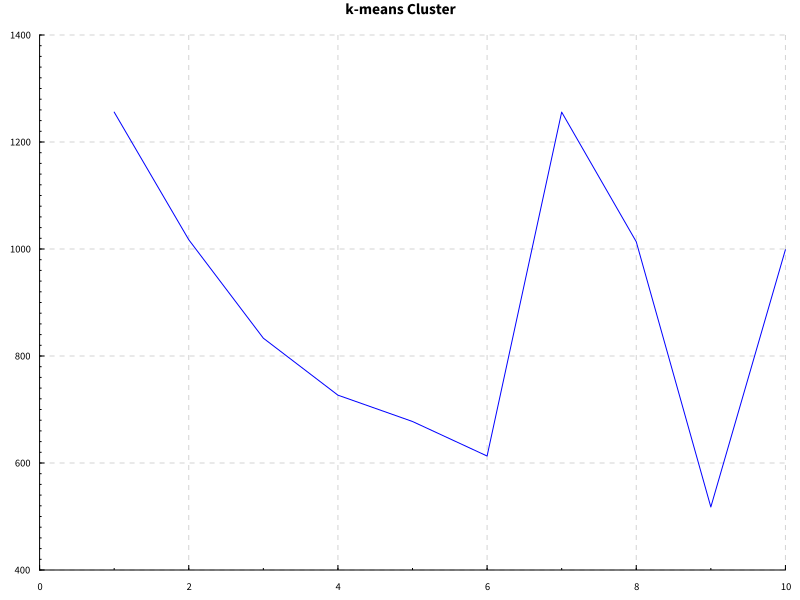
\includegraphics[width=0.7\textwidth]{elbow}
  \caption{Elbow Plot of the \textit{WCSS} dependening on $k$.}
\label{fig:elbow}
\end{figure}

\begin{figure}[h]
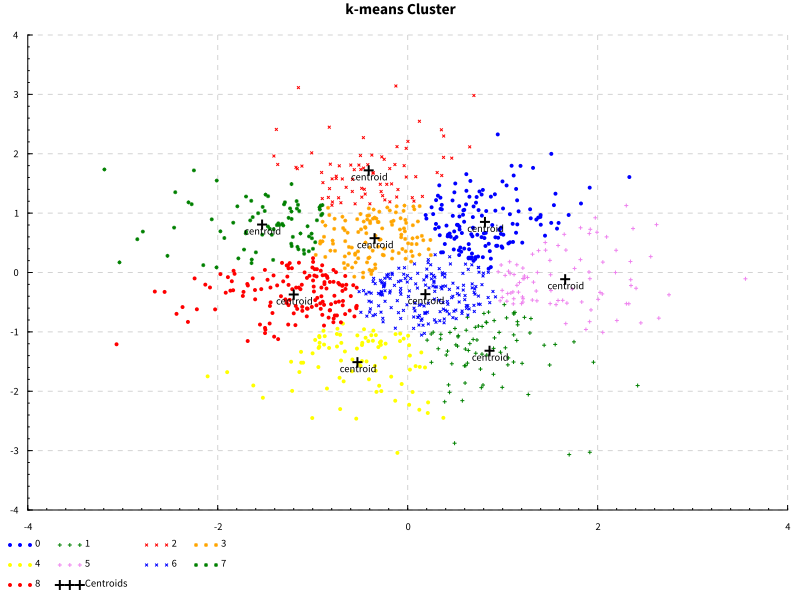
\includegraphics[width=1\textwidth]{kmeans}
\centering
\caption{Example of $k$-means clustering for 100,000 observations.}
\label{fig:kmeans}
\end{figure}

\subsection{Complexity}\label{s:algo}

The complexity of the standard algorith in $d$-dimensions is $\mathcal{O}(t \cdot n \cdot k \cdot d)$, where $t$ is the number of iterations until local optimum, $n$ is the number of observations, $k$ is the number of clusters, and $d$ is the number of dimensions.

\section{The code}\label{s:intro}

\subsection{Implementation}\label{s:intro}

The first implementation of the algorithm from \textit{pseudo-code} to real code took performance into consideration by using an array-like data structure (from the library \code{vector}) and points was represented in an efficient way by using \textit{unboxed} types (types that are represented by words in registers instead of pointers). The code can be found at \code{KMeans0.hs}.

After finishing the first implementation, we wanted to measure its performance using a consistent and objective method. We used a well-known benchmark framework called \code{criterion} \cite{criterion}. We wrote a couple of benchmarks, see \code{Benchmark.hs}. The initial results were not good as it took more than one minute to process less than $5,000$ $2$-dimensional points.

\newpage

In order to see what was making the implementation so slow, we wrote a simple program (see \code{./profile/Main0.hs}) and we used GHC's profiling capabilities \cite{ghc_profiling} to generate a \textit{prof} file which contained detailed statistics of the execution time, garbage collection pauses, execution trace, etc. \code{profiteur} \cite{profiteur} is a nice tool for visualizing the \textit{prof} files which are usually long and hard to read.

\begin{figure}[h]
\includegraphics[width=1\textwidth]{profiteur}
\centering
  \caption{profiteur, graphic visualization of \textit{prof} files.}
\label{fig:profiteur}
\end{figure}

\subsection{Optimizations}\label{s:intro}

The profiling gave us some hints about were was the bottleneck (see Figure \ref{fig:profile}). As you may see, the garbage collector (GC) is taking up to half of the execution time so this is probably due to a spaceleak which is a known problem of lazy evaluation. Spaceleaks are hard to find but easy to solve. We followed a novel technique to find where the memory was being accumulated by restricting the maximum amount of stack. After finding where the memory was leaking, we forced the evaluation of the big thunk of memory to avoid the garbage collector going ill. To apply strictness in some points of the code, we used the great haskell extension \code{BangPatterns} which gives a nice sugar-syntax to call \code{seq and deepseq} primitives to force evaluation.

\begin{figure}[H]
\includegraphics[width=0.9\textwidth]{profile}
\centering
  \caption{Profile statistics from GHC's profiling.}
\label{fig:profile}
\end{figure}

Apart from fixing the spaceleak that gave us a huge speed-up, we applied some microoptimizations to the hot spots of our algorithm that are the \code{euclideanDistance} function and the \code{constructCluster} function.

Figure \ref{fig:bench} displays the final results for different values of $n$ (observations) and $k$ (clusters). For a better visualization, open \code{./bench/bench.html} in your favourite browser and play with the interactive plots and nice statistics produced by \code{criterion}.

\begin{figure}[H]
\includegraphics[width=1\textwidth]{bench}
\centering
  \caption{Benchmark of \code{KMeans0} and \code{KMeans1}.}
\label{fig:bench}
\end{figure}

\section{Conclusions \& Future Work}\label{s:conclusions}

This project described and implemented an optimized \textit{standard k-means clustering algorithm} in Haskell by applying low-level optimitizations, also known as \textit{micro-optimizations}, such as strict annotations and inlineable code. This process required to understand Haskell evaluation and performance issues. We got assistance from really great tools to profile and benchmark our application and the result is quite good compared to the first implementation.

A major speed-up can be achieved by implementing a more efficient version of your algorithm. For example, C.M. Poteras et al. proposed an optimized version of the K-Means clustering algorithm which achieves an observable speed up of $1.7x$ on large data sets \cite{optimized}. Implementing the optimized algorithm \ref{algo:optimized} in Haskell is feasible and an interesting task for future work.

\begin{algorithm}[H]
  1. Defined constant $W\!I\!D\!T\!H$ \\
  2. Define intervals $I_i = [i*W\!I\!D\!T\!H, (i+1)*W\!I\!D\!T\!H]$ and tag them with value $i * W\!I\!D\!T\!H$ \\
  3. Mark the entire data set to be visited \\
  4. For each point to be visited \\
  5. Compute $e = min(d_{PC_l} - d_{PC_w})$ where $C_w$ is the center of the winner (closest) cluster and $C_l, l = 1..k, l \neq w$ stands for all other centroids. \\
  6. Map all points with $i * W\!I\!D\!T\!H < e < (i+1)*W\!I\!D\!T\!H$ to interval $i * W\!I\!D\!T\!H$ where $i$ is a positive integer. \\
  7. Compute new centroids $C_j$, where $j = 1..k$ and their maximum deviation $D = max(|C_jC_{j'}|)$ \\
  8. Update $I_j$'s tag by substracting $2*D$ (points owned by this interval go closer to the edge by $2*D$) \\
  9. Pick up all points inside intervals whose tag is less or equal to 0, and go to 4 to revisit them.
  \caption{Optimized K-Means algorithm}
  \label{algo:optimized}
\end{algorithm}

%%%%%%%%%%%%%%%% BIBLIOGRAPHY %%%%%%%%%%%%%%%%%%%%%

\bibliographystyle{alpha} % abbrv, aplha, plain, abstract, apa, unsrt,
\bibliography{refs}

\end{document}
